\chapter{Results}
This chapter demonstrates that the communication between the Client and Server is encrypted as expected, as well as the obtained performance on the ESP32 board.
All issues identified during the project's development are reported and explained. A small section with possible future works is also described.    

\section{Encrypted communication checking}
After developing the project application, the packets sent during the communication where analysed through WireShark \cite{WireShark}, which is a free and open source packets analyser.
In this way it was possible to test that the interaction between the ESP32 and the user was really under a VPN protocol, and so correctly encrypted.\\
Below there are two WireShark capture: in these the packet that was captured was the one containing the user password, because it is the most vulnerable data exchanged.

\begin{itemize}
    \item In Figure \ref{fig:WSpublic} there is the capture of the packet in the public network.\\It could be seen that the source and destination IPs are the one of the physical devices, and the communication is happening under a WireGuard protocol.\\Moreover the content of the packets is not visible, and so it has been successfuly encrypted.
    \item In Figure \ref{fig:WSwg} there is the capture of the packet in the WireGuard Network Interface.\\In this case the source and destination IPs are the one assigned by WireGuard Interface, and it could be seen that the packet sent is exactly the user password, so the packet exchange during the communication is the correct one.\\
\end{itemize}

\begin{figure}[H]
    \centering
    \vspace{0.5cm}
    \includegraphics[width=\textwidth, scale=0.25]{images/WS\_publicNet.png}
    \caption{WireShark capture public Network}
    \label{fig:WSpublic} % This is the image label, with which you can refer to the image in any document location.
\end{figure}

\begin{figure}[H]
    \centering
    \vspace{0.5cm}
    \includegraphics[width=\textwidth, scale=0.25]{images/WS\_wgNet.png}
    \caption{WireShark capture WireGuard Network Interface}
    \label{fig:WSwg} % This is the image label, with which you can refer to the image in any document location.
\end{figure}

\section{Performance and resource consumption}\label{sec:performance}
No performance measurements were made on the FreeRTOS simulator for Linux, since it is very different from an actual embedded device.
Program sizes are also influenced by C library code needed to interface with the host, since the whole simulation is compiled into a single executable file.
\\Performance was evaluated on the ESP32 platform using the \texttt{iperf} port provided in the \texttt{ESP-IDF} SDK with the \texttt{wireguard-lwip} module added, see chapter \ref{sec:iperf_wg}.
\\The WiFi network was too slow in the experiments conducted to determine if the cryptography was CPU bound. The best throughput achieved was 11 Mbit/s both directions, both inside and outside the WireGuard tunnel.\\
While this result is not conclusive, it clears the envelope for many applications with limited bandwidth requirements.
Also, many real-world scenarios replicate the same conditions yielding the same or much worse link speeds.
All in all, the communication will not be CPU-bound in most practical cases.
\\Resource consumption was low enough for the ESP32, although this should be evaluated for each platform.\\
37 kilobytes of ROM are needed for the WireGuard module, including the very basic configuration command described in the dedicated chapter. This was deduced from binary sizes at compile time: \texttt{idf.py build} reports a number of used bytes in hexadecimal after the build is complete.\\
For an ESP32 this should be an acceptable quantity of flash for most projects, especially considering the operating system requires 600 kB of flash.
\begin{figure}[H]
    \centering
    \vspace{0.5cm}
    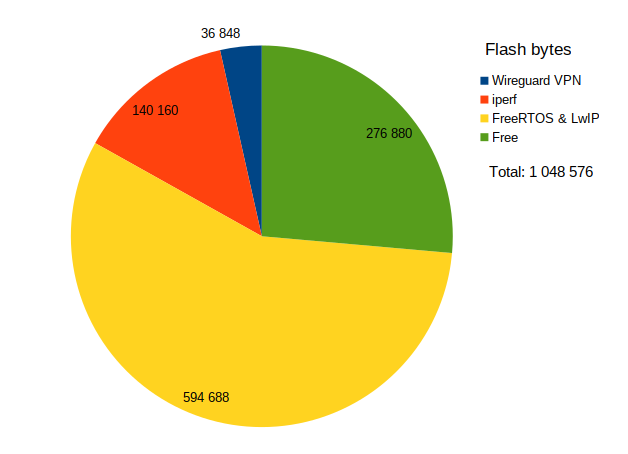
\includegraphics[width=0.5\textwidth, scale=0.25]{images/iperf_flash_footprint.png}
    \caption{iperf with WireGuard: flash memory footprint contributions}
    \label{fig:iperf_flash_piechart} % This is the image label, with which you can refer to the image in any document location.
\end{figure}

RAM heap usage on the ESP32 was 1700 bytes at idle and 7 kilobytes while running iperf. This was reported using the \texttt{free} and \texttt{heap} commands available in the serial console of the iperf port, see \ref{sec:iperf_wg} and \ref{fig:iperf_wg_long}.\\
The ESP32 has 500 kB of internal RAM, of which 220 kB are usable by applications.

\section{Known Issues}\label{sec:problems}
This report shows how to set up a basic VPN tunnel using WireGuard on different cases, however some issues were left unfixed.
\begin{itemize}
    \item Every procedure described works as intended on Linux systems only. On Windows platforms WSL is available, however it does not provide a complete Linux system, and a common virtual machine could be more useful. Most notably:
    \begin{itemize}
        \item WSL 2 is basically a virtual machine, so networking is more complicated (a virtual interface connects to the internet through NAT, \textbf{hyper-v virtual ethernet adapter} issues) and no server can easily run from inside the VM. Also connecting serial devices (which is needed to flash a firmware onto ESP32 chips) requires setting up USB pass-through every time the device is plugged in, which sums up to one command in the Windows host and one command inside WSL.
        \item WSL 1 offers better compatibility. There were no problems with networking, but USB devices problem still remain. It is hard to fix and even so, the build process was really slow (10-15 min on a performant machine). 
        \item Oracle VirtualBox was most practical, offering one-click USB pass-through configuration, and bridged networking that was functional over WiFi too.
    \end{itemize}
    Networking was especially important, because some tools (most notably Netcat) are missing in Windows.
    
    \item 32 bit \texttt{sys\_now()} timestamp: on most LwIP platforms the TAI64N timestamp necessary for WireGuard is obtained from the \texttt{sys\_now()} function of LwIP that returns a 32 bit unsigned millisecond count that overflows every 49 days. The timestamp is always between 01/01/1970 and 18/02/1970. While it is not a problem that the date is far in the past, when the timestamp overflows, or when the device reboots, the date and time go back to a previous instant (01/01/1970). The WireGuard server will reject all handshake packets with an earlier timestamp than the last received, so communication will not be possible until the server is killed and restarted.
    
    \item The random number generator used in the Linux simulator port is not cryptographically secure. 
    See the \texttt{rand()} call inside \texttt{wireguard\_random\_bytes()} in file 
    \begin{lstlisting}
    wireguard-lwip/src/wireguard-platform_unix_freertos.c
    \end{lstlisting}
    Although security was not needed for the simulation, it should be clear that this flaw compromises the whole cryptosystem. A strong random number generator should be implemented for any practical application, as was done for the port to the ESP32 platform.
    
    \item A large number of TCP retransmissions is sometimes generated by the peer using the \textbf{wireguard-lwip} module, usually for an interval of up to 10 seconds, even in perfect conditions (like TAP networking). While performance is very good, this issue should probably be addressed before a practical application is deployed, as there is the potential for some important flaw to be the cause of such a seemingly random malfunction.
    \item All the test on the esp32 have been done using the ESP-IDF version 4.4.1. The latest version available at the time of writing this paper (v5.0.0) does not work with the presented project.
\end{itemize}

\section{Future Works}

The following two important steps are still missing to produce a usable solution:
\begin{itemize}
    \item User friendly configuration of the VPN keys and static IPs. This can be added along the configuration of the WiFi access parameters, keeping in mind that it may not be practical to type two 44-character long keys on a small keyboard or on a number-only keyboard.
    \item Internet routing was not tested nor desired for this project, communication with a single computer was enough. While potentially no changes to the \texttt{wireguard-lwip} module may be needed, the configuration becomes more involved on any peer that has to route traffic to other hosts inside the VPN, be it on a physical local network or to other connected WireGuard peers.
\end{itemize}


